\documentclass[aps,prl,twocolumn,superscriptaddress,nofootinbib]{revtex4-2}

\usepackage[utf8]{inputenc}
\usepackage[T1]{fontenc}
\usepackage{amsmath,amssymb}
\usepackage{graphicx}
\usepackage{booktabs}
\usepackage{siunitx}
\usepackage{hyperref}
\usepackage{xcolor}

\graphicspath{{./}{data_analysis/week_1/results/}{data_analysis/week_2/results/}{data_analysis/combined_analysis/results/}}

\begin{document}

\title{Effective Attenuation of Cosmic-Ray Coincidence Events in Lead Absorbers}

\author{Student Name}
\affiliation{Department / Laboratory, Institution}

\date{\today}

\begin{abstract}
We analyze a two-scintillator cosmic-ray coincidence experiment with lead absorbers placed between the upper and lower detectors. Events are selected using a fixed pulse-integral threshold, $(\mathrm{area}>30)\land(\mathrm{area2}>30)$. Week-1 data cover 0--30 lead plates and show a consistent decrease in the effective coincidence rate. Week-2 data cover 0, 40, 50, and 60 plates, but exhibit clear detector-response changes, especially in the lower detector channel. We compare absolute coincidence rates, normalized conditional coincidence ratios, and zero-lead scaled rates. The results show that the measured attenuation is an effective coincidence attenuation determined by lead scattering, detector geometry, threshold response, and detector efficiency, rather than a pure muon absorption length in lead.
\end{abstract}

\maketitle

\section{Introduction}

Cosmic rays reaching sea level are dominated by secondary particles produced when primary cosmic rays interact with the atmosphere. The charged component relevant to this experiment is mainly composed of muons, which are produced through pion and kaon decay chains. Their relativistic energy and time dilation allow many of them to reach ground level before decaying.

The angular distribution of near-vertical sea-level muons can be approximated as
\begin{equation}
I(\theta) \simeq I(0)\cos^2\theta,
\end{equation}
so a pair of vertically aligned scintillation detectors acts as a simple geometrical telescope for near-vertical cosmic-ray events.

The objective of this experiment is to measure how the two-detector coincidence rate changes as lead absorber thickness increases. Because the detectors have finite area and a fixed threshold, the measured quantity is not a pure absorption probability. Instead, it is an effective coincidence probability affected by ionization loss, multiple scattering, detector geometry, and detector efficiency.

\section{Experimental Principle}

Each event contains pulse-integral quantities from the upper and lower detectors:
\begin{equation}
\mathrm{area}\quad \mathrm{and}\quad \mathrm{area2}.
\end{equation}
The fixed event-selection condition is
\begin{equation}
\mathrm{coincidence} = (\mathrm{area}>30)\land(\mathrm{area2}>30).
\end{equation}
We define
\begin{align}
N_{\rm up} &= \#(\mathrm{area}>30),\\
N_{\rm down} &= \#(\mathrm{area2}>30),\\
N_{\rm coin} &= \#[(\mathrm{area}>30)\land(\mathrm{area2}>30)].
\end{align}
The coincidence rate is
\begin{equation}
R_{\rm coin}=\frac{N_{\rm coin}}{T},
\end{equation}
with $T=\SI{3600}{s}$ and timing uncertainty $\sigma_T=\SI{60}{s}$.

The relative uncertainty is taken as
\begin{equation}
\frac{\sigma_R}{R_{\rm coin}}=
\sqrt{\frac{1}{N_{\rm coin}}+\left(\frac{\sigma_T}{T}\right)^2}.
\end{equation}

We also use the conditional coincidence ratio
\begin{equation}
\frac{N_{\rm coin}}{N_{\rm up}},
\end{equation}
which estimates the probability that an upper-detector candidate also passes the lower-detector threshold. This quantity is useful for inter-week comparison, but it is still sensitive to the lower detector response.

The effective transmission and blocking are defined as
\begin{align}
\mathcal{T}(x) &= \frac{R_{\rm coin}(x)}{R_{\rm coin}(0)},\\
\mathcal{B}(x) &= 1-\mathcal{T}(x).
\end{align}
Here $\mathcal{B}$ is an effective blocking fraction, not a pure muon absorption probability.

\section{Data Sets and Processing}

The data were collected in two measurement weeks. Week 1 contains 0, 10, 20, and 30 lead plates, corresponding to 0, 5, 10, and \SI{15}{mm}. Week 2 contains 0, 40, 50, and 60 lead plates, corresponding to 0, 20, 25, and \SI{30}{mm}.

The ROOT files were preprocessed into NumPy arrays using \texttt{uproot}. The analysis uses the event-level scalar branches \texttt{area}, \texttt{area2}, \texttt{amp}, \texttt{base}, \texttt{rms}, and \texttt{Index\_minamp}.

\section{Attenuation Fits}

Two empirical exponential models are used. The first fits the normalized transmission:
\begin{equation}
\mathcal{T}(x)=\exp(-x/\lambda_{\rm eff}).
\end{equation}
The second fits the absolute coincidence rate:
\begin{equation}
R_{\rm coin}(x)=R_0\exp(-x/\lambda_{\rm eff}).
\end{equation}
The parameter $\lambda_{\rm eff}$ is an effective attenuation length in the current detector geometry and threshold configuration. It should not be interpreted as the true muon absorption length in lead.

\section{Week-1 Results}

Week 1 shows a consistent decrease in effective coincidence rate as lead thickness increases. The fixed-threshold coincidence counts are summarized in Table~\ref{tab:week1}.

\begin{table}[h]
\caption{Week-1 coincidence statistics.}
\label{tab:week1}
\begin{ruledtabular}
\begin{tabular}{cccc}
Run & Plates & $N_{\rm coin}$ & $\mathcal{T}$\\
\hline
5181 & 0  & 3357 & 1.000\\
5182 & 10 & 3136 & 0.934\\
5183 & 20 & 3119 & 0.929\\
5184 & 30 & 3046 & 0.907\\
\end{tabular}
\end{ruledtabular}
\end{table}

\begin{figure}[h]
\centering
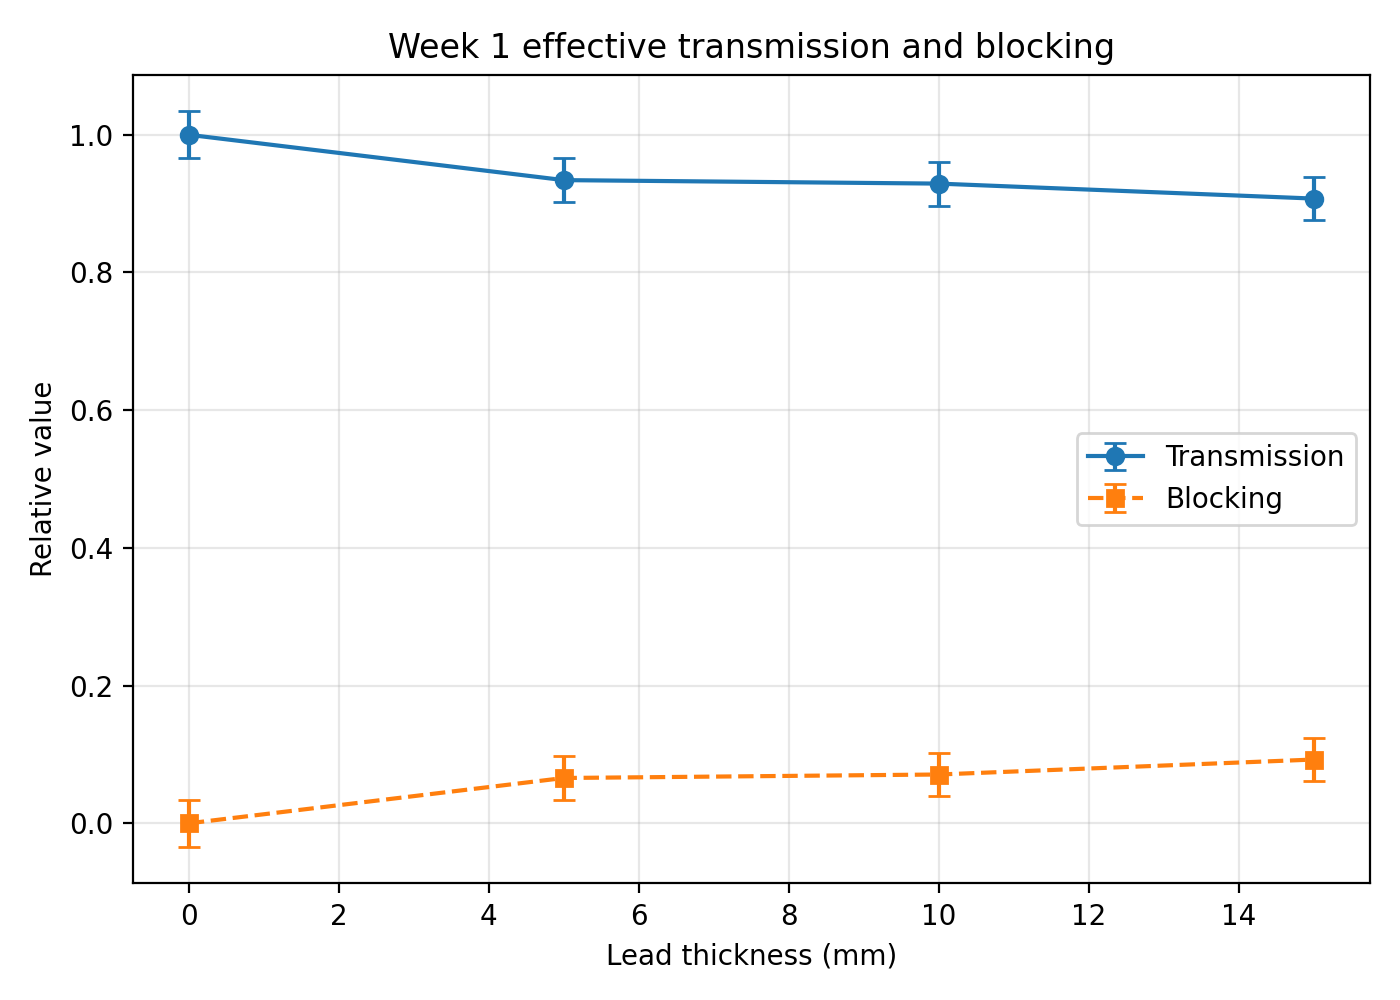
\includegraphics[width=\linewidth]{figures/week1_transmission_blocking.png}
\caption{Week-1 effective transmission and blocking as functions of lead thickness.}
\label{fig:week1_transmission}
\end{figure}

The Week-1 transmission fit gives
\begin{equation}
\lambda_{\rm eff} = (137.45 \pm 34.85)\ \mathrm{mm},
\end{equation}
with $\chi^2/{\rm ndf}=0.335$. The absolute coincidence-rate fit gives
\begin{equation}
\lambda_{\rm eff} = (168.09 \pm 62.02)\ \mathrm{mm},
\end{equation}
with $\chi^2/{\rm ndf}=0.701$.

\begin{figure}[h]
\centering
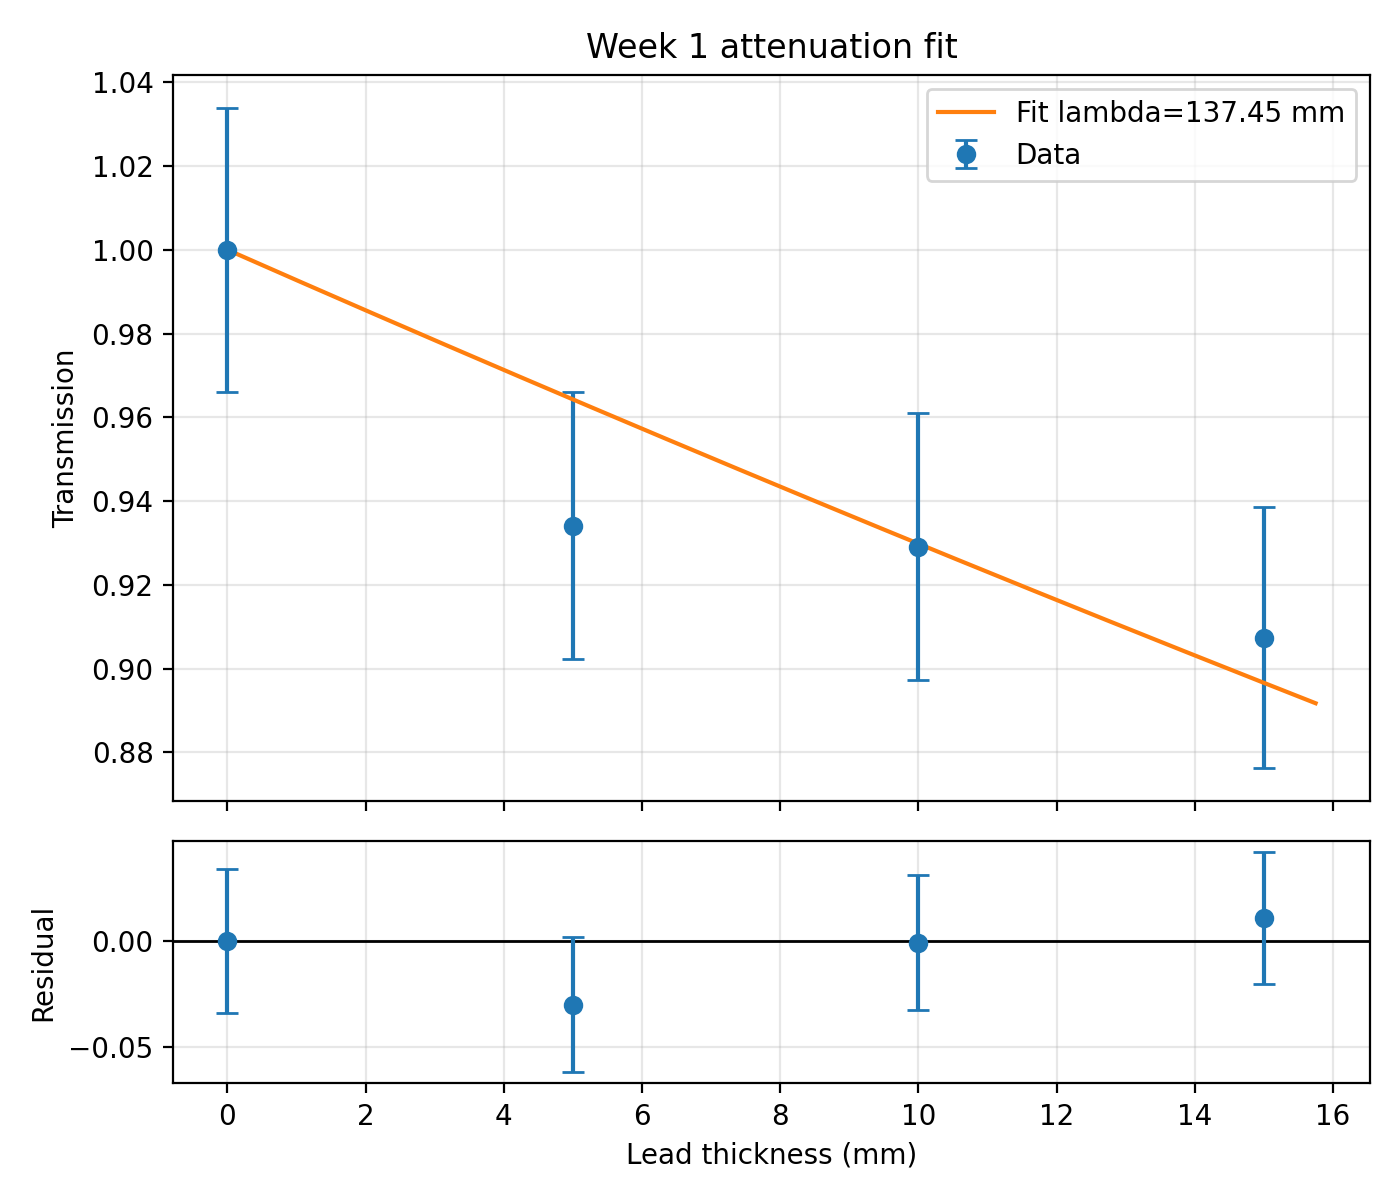
\includegraphics[width=\linewidth]{fit/week1_attenuation_fit.png}
\caption{Week-1 exponential fit to normalized transmission.}
\label{fig:week1_fit}
\end{figure}

\section{Week-2 Results}

Week 2 does not show a clean monotonic attenuation trend. The fixed-threshold coincidence counts are summarized in Table~\ref{tab:week2}.

\begin{table}[h]
\caption{Week-2 coincidence statistics.}
\label{tab:week2}
\begin{ruledtabular}
\begin{tabular}{cccc}
Run & Plates & $N_{\rm coin}$ & $\mathcal{T}$\\
\hline
51811 & 0  & 1831 & 1.000\\
5185  & 40 & 1523 & 0.832\\
5186  & 50 & 1579 & 0.862\\
5187  & 60 & 1687 & 0.921\\
\end{tabular}
\end{ruledtabular}
\end{table}

The Week-2 transmission fit gives $\lambda_{\rm eff}=(188.23\pm33.90)\,\mathrm{mm}$ with $\chi^2/{\rm ndf}=2.384$, while the absolute rate fit gives $\lambda_{\rm eff}=(239.47\pm75.59)\,\mathrm{mm}$ with $\chi^2/{\rm ndf}=6.364$. The relatively poor agreement, especially for the absolute rate fit, indicates significant systematic effects.

\begin{figure}[h]
\centering
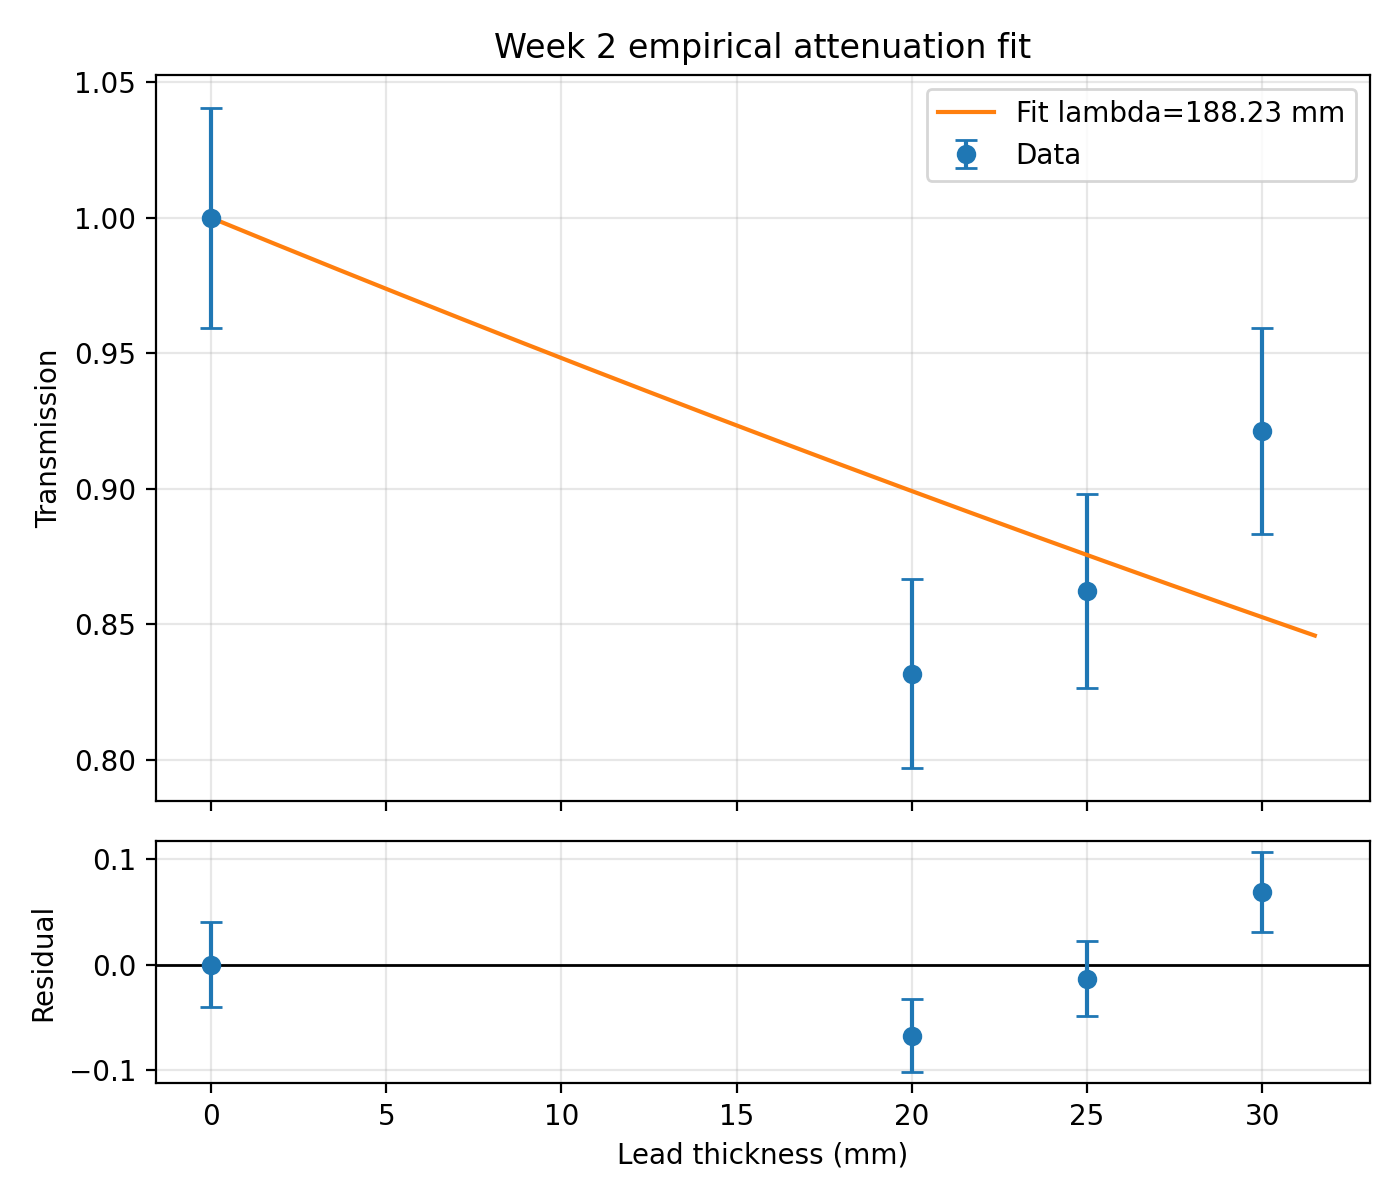
\includegraphics[width=\linewidth]{fit/week2_attenuation_fit.png}
\caption{Week-2 empirical exponential fit to normalized transmission. The fit is used only as a trend estimate because Week-2 data show detector-response changes.}
\label{fig:week2_fit}
\end{figure}

\section{Inter-Week Consistency}

The zero-lead baselines differ strongly:
\begin{equation}
N_{\rm coin}^{\rm W1}(0)=3357,\qquad
N_{\rm coin}^{\rm W2}(0)=1831.
\end{equation}
The Week-2 baseline is only about $0.545$ of the Week-1 baseline.

The detector response also changes significantly. In the zero-lead data, the lower-detector mean pulse integral shifts from $34.74$ in Week 1 to $17.71$ in Week 2. Consequently, the fixed lower-channel threshold $\mathrm{area2}>30$ becomes more restrictive in Week 2.

\begin{figure}[h]
\centering
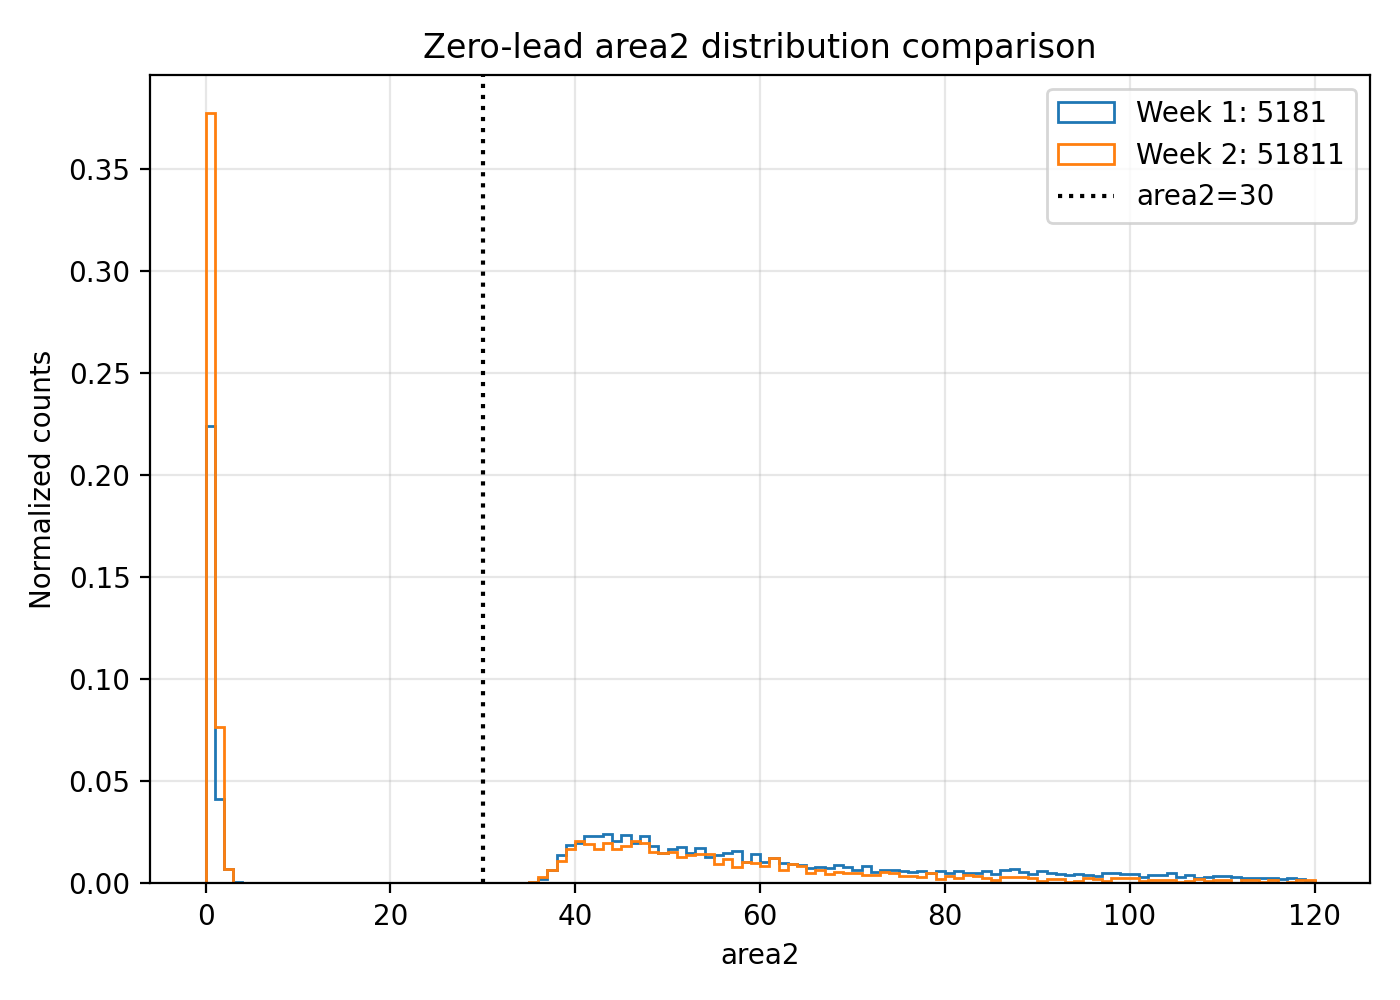
\includegraphics[width=\linewidth]{figures/zero_lead_area2_comparison.png}
\caption{Comparison of the lower-detector pulse-integral distribution for the zero-lead baselines. The Week-2 distribution is shifted to lower values, indicating detector-response drift.}
\label{fig:area2_shift}
\end{figure}

\section{Combined Normalization}

To compare the full 0--60 plate range, a zero-lead scale factor is defined:
\begin{equation}
k=\frac{R_{\rm coin}^{\rm W1}(0)}{R_{\rm coin}^{\rm W2}(0)}
=\frac{3357}{1831}=1.833.
\end{equation}
The scaled Week-2 rates are then
\begin{equation}
R_{\rm coin,scaled}^{\rm W2}(x)=kR_{\rm coin}^{\rm W2}(x).
\end{equation}

\begin{table}[h]
\caption{Zero-lead scaled 0--60 plate trend.}
\label{tab:combined}
\begin{ruledtabular}
\begin{tabular}{cccc}
Run & Plates & Scaled counts/hour & Scaled $\mathcal{T}$\\
\hline
5181 & 0  & 3357.0 & 1.000\\
5182 & 10 & 3136.0 & 0.934\\
5183 & 20 & 3119.0 & 0.929\\
5184 & 30 & 3046.0 & 0.907\\
5185 & 40 & 2792.3 & 0.832\\
5186 & 50 & 2895.0 & 0.862\\
5187 & 60 & 3093.0 & 0.921\\
\end{tabular}
\end{ruledtabular}
\end{table}

\begin{figure}[h]
\centering
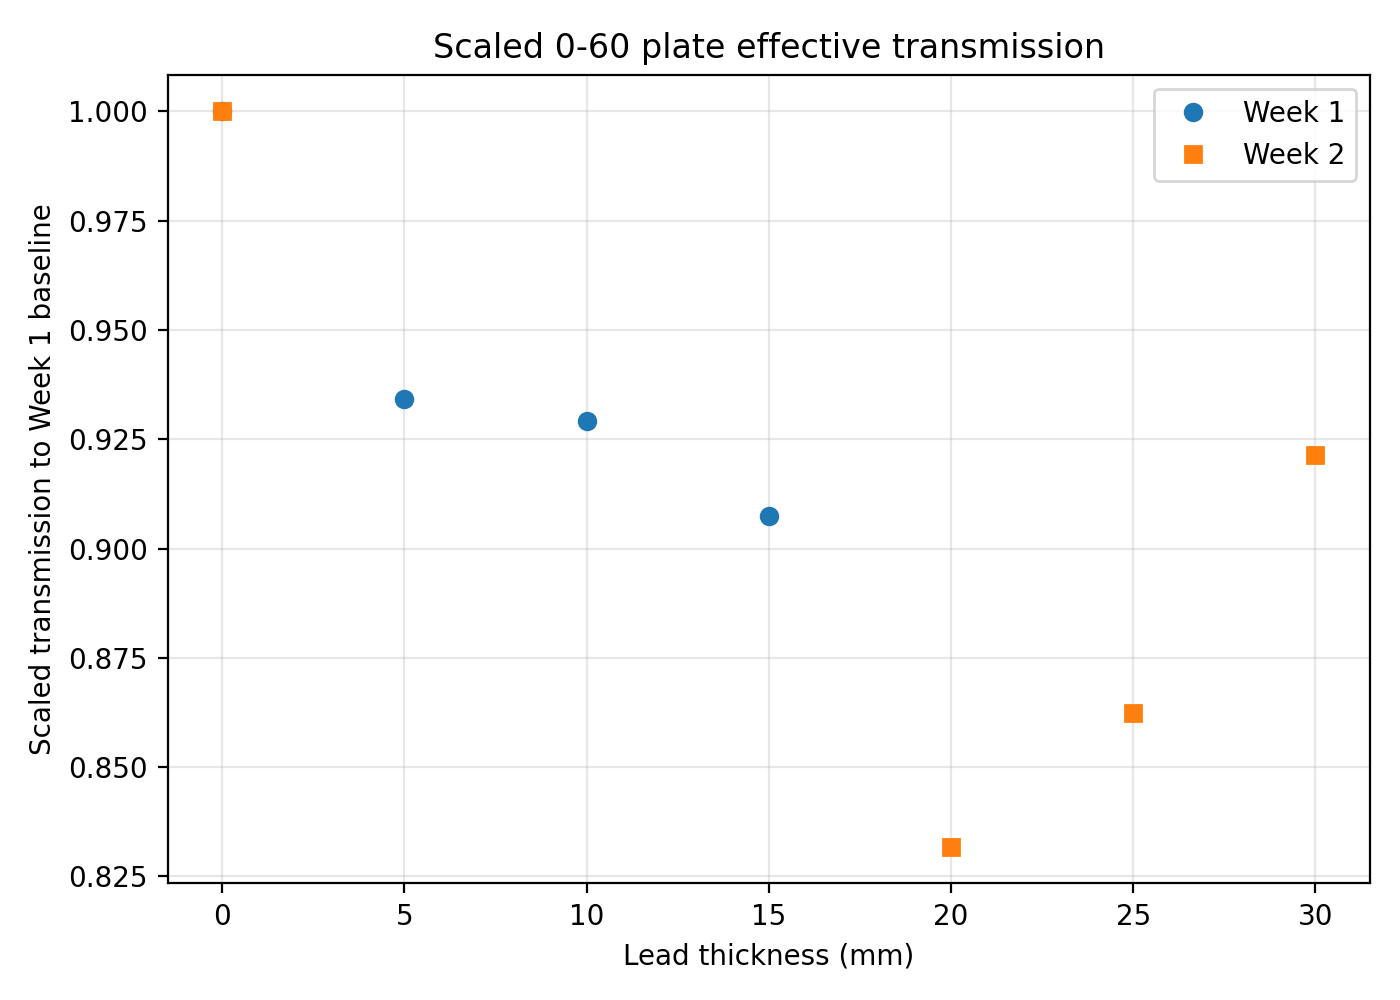
\includegraphics[width=\linewidth]{figures/scaled_transmission_combined.png}
\caption{Zero-lead scaled effective transmission over the full 0--60 plate range. The non-monotonic Week-2 thick-lead points show that a single scale factor cannot fully remove inter-week systematic effects.}
\label{fig:combined_scaled}
\end{figure}

\section{Discussion}

The Week-1 results are compatible with an effective attenuation trend. The Week-2 results, however, show non-monotonic thick-lead behavior and clear detector-response changes. The inter-week shift in the zero-lead baseline and in the lower-detector pulse-integral distribution indicates that absolute rates cannot be directly concatenated.

The scaled 0--60 plate curve is useful as a diagnostic visualization, but it should not be interpreted as a clean global attenuation measurement. A more conservative interpretation is to report Week 1 and Week 2 separately, then use zero-lead scaling and conditional coincidence ratios such as $N_{\rm coin}/N_{\rm up}$ to estimate the size of systematic effects.

\section{Conclusion}

We measured the effective attenuation of cosmic-ray coincidence events in lead absorbers using a two-scintillator detector system. Week 1 shows a consistent decrease in coincidence rate with lead thickness and yields an effective attenuation length of order $10^2\,\mathrm{mm}$. Week 2 shows detector-response drift, especially in the lower detector channel, and cannot be treated as a clean attenuation curve. After zero-lead scaling, the combined 0--60 plate trend remains non-monotonic in the thick-lead region, demonstrating that detector-response systematics must be included. The experiment therefore measures an effective coincidence attenuation, not the pure absorption length of cosmic-ray muons in lead.

\begin{thebibliography}{99}

\bibitem{pdg_cosmic}
Particle Data Group, ``Cosmic Rays,'' \textit{Review of Particle Physics} (2024).

\bibitem{pdg_matter}
Particle Data Group, ``Passage of Particles Through Matter,'' \textit{Review of Particle Physics} (2024).

\bibitem{rossi1933}
B. Rossi, ``Interaction between Cosmic Rays and Matter,'' \textit{Nature} \textbf{132}, 173 (1933).

\bibitem{rossi_book}
B. Rossi, \textit{High-Energy Particles} (Prentice-Hall, 1952).

\bibitem{caen}
CAEN, ``DT5742 Digitizer Documentation,'' \url{https://www.caen.it/products/dt5742/}.

\end{thebibliography}

\end{document}

